\documentclass[problem]{mcs}

\begin{pcomments}
  \pcomment{CP_planar_embedding_isomorphism}
  \pcomment{from: S09.cp7m, S07.cp7m}
\end{pcomments}

\pkeywords{
  planar_graphs
  planar_embeddings
  discrete_face
  face
  isomorphism
  recursive
}

%%%%%%%%%%%%%%%%%%%%%%%%%%%%%%%%%%%%%%%%%%%%%%%%%%%%%%%%%%%%%%%%%%%%%
% Problem starts here
%%%%%%%%%%%%%%%%%%%%%%%%%%%%%%%%%%%%%%%%%%%%%%%%%%%%%%%%%%%%%%%%%%%%%

\begin{problem}
Figures 1--4 show different pictures of planar graphs.
\begin{figure}[h]\redrawn
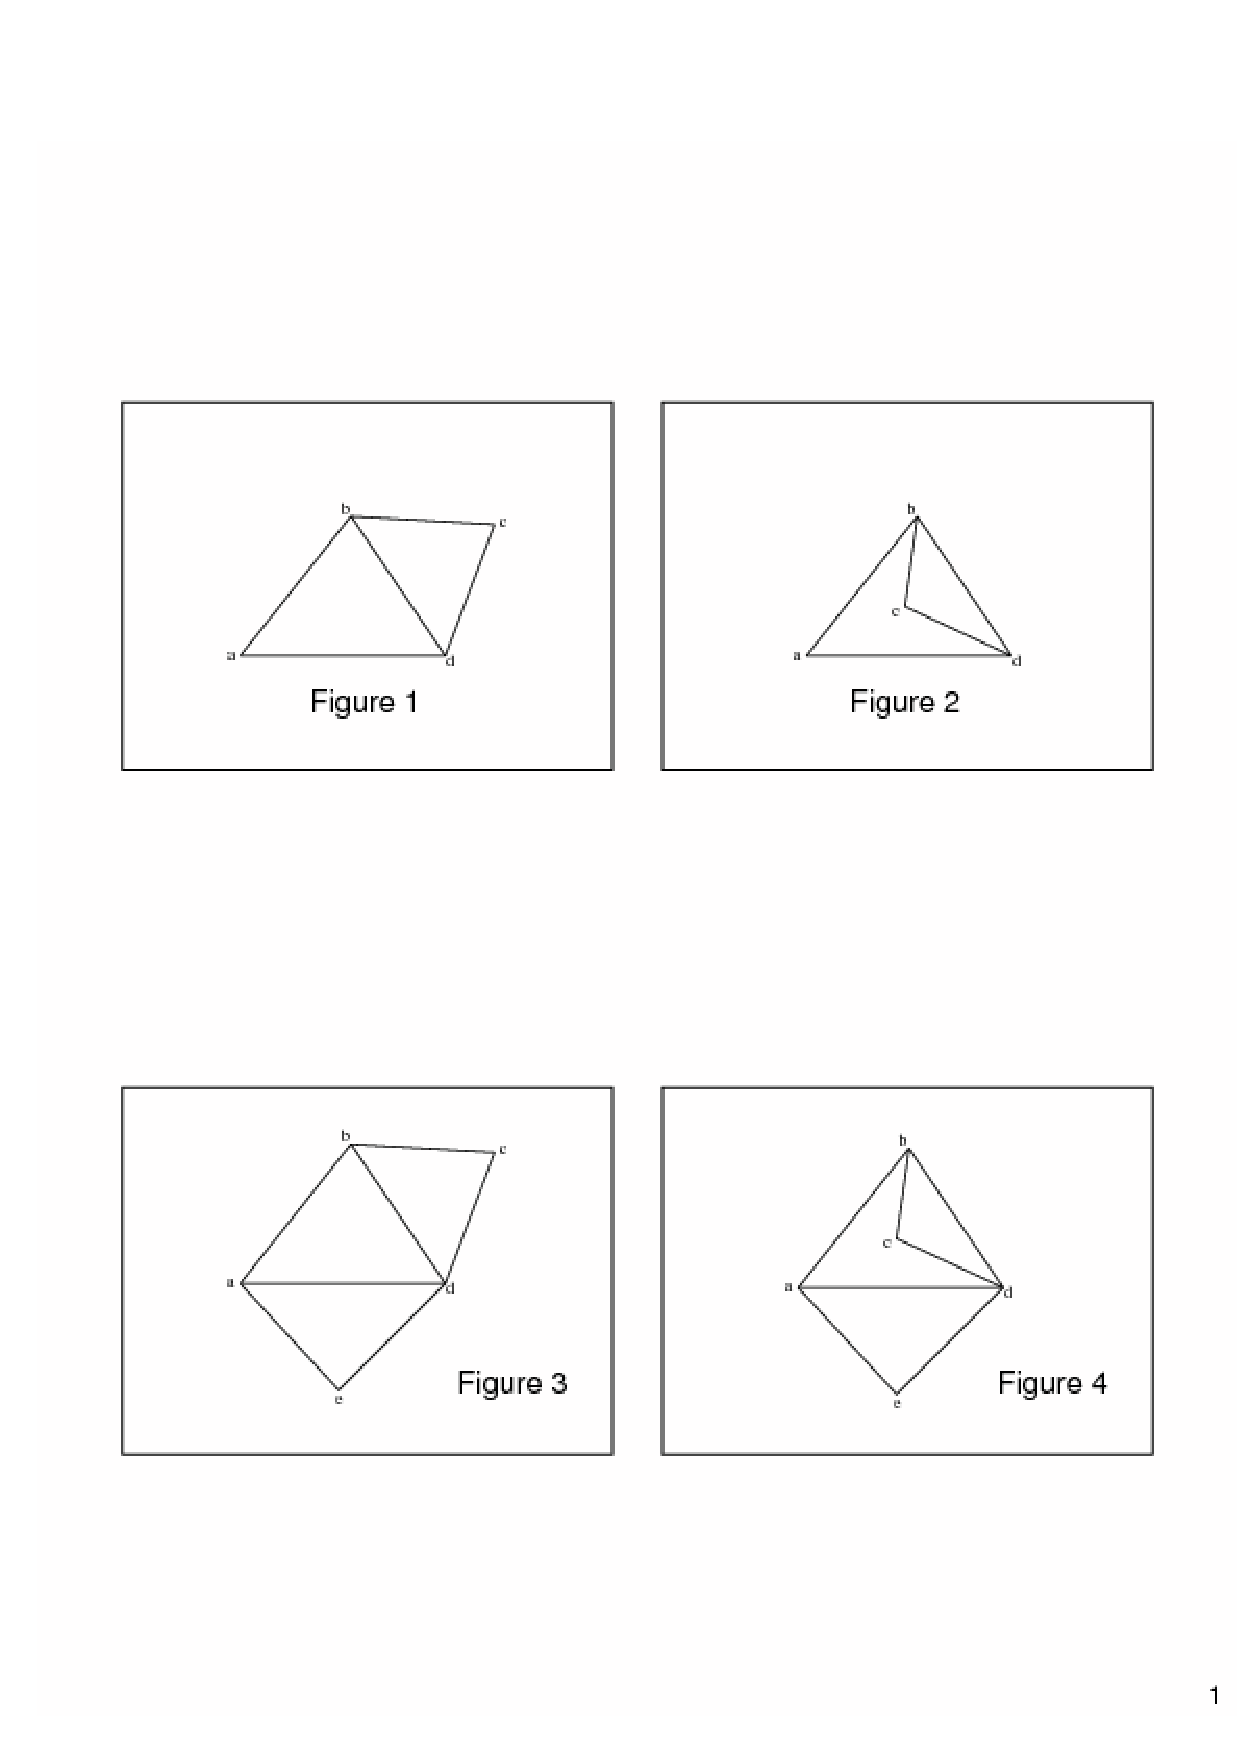
\includegraphics{cp7mfigs-new}
\end{figure}

\begin{staffnotes}
Letters labelling vertices are hard to read.  Make sure you know what
they are.  A better figure would be appreciated.
\end{staffnotes}
        
\bparts

\ppart For each picture, describe its discrete faces (simple cycles that
define the region borders).

\begin{solution}
Figs 1 \& 2: abda, bcdb, abcda.
Fig 3: abcdea, adea,abda,bcdb.  Fig 4: abcda, abdea, bdcb, adea.
\end{solution}

\ppart Which of the pictured graphs are isomorphic?  Which pictures
represent the same \emph{planar embedding}? -- that is, they have the same
discrete faces.

\begin{solution}
  Figs 1 \& 2 have the same faces, so are different pictures of the
  \emph{same} planar drawing.  Figs 3 \& 4 both have four faces, but they
  are different, for example, Fig 3 has a face with 5 edges, but the
  longest face in Fig 4 has 4 edges.
\end{solution}

\ppart Describe a way to construct the embedding in Figure 4 according to
the recursive Definition~\bref{embeddingdef} of planar embedding.  For
each application of a constructor rule, be sure to indicate the faces
(cycles) to which the rule was applied and the cycles which result from
the application.

\begin{solution}
  Here's one way.  (By Lemma~\bref{switch-edges}, the constructor steps
  could be done in any order.)

\begin{staffnotes}
Make sure students write out the full set of faces at each step as in the solution below.
\end{staffnotes}

\[\begin{array}{ccr}
\text{recursive step} & & \text{faces}\\\hline
\text{vertex } a & \text{(base case)} & a\\
\text{vertex } b & \text{(base)} & b\\
\edge{a}{b} & \text{(bridge)} & aba\\
\text{vertex } c & \text{(base)} & c\\
\edge{b}{c} & \text{(bridge)} & abcba\\
\text{vertex } d & \text{(base)} & d\\
\edge{c}{d} & \text{(bridge)} & abcdcba\\
\edge{a}{d} & \text{(split)} & dabcd,\ dabcd\\
\edge{b}{d} & \text{(split)} & dabd,\ dbcd,\  abcda\\
\text{vertex } e & \text{(base)} & e\\
\edge{d}{e} & \text{(bridge)} & dedabd,\ dbcd,\  abcda\\
\edge{a}{e} & \text{(split)}  & abdea,\ adea,\ dbcd,\ abcda\\
\end{array}\]

\end{solution}

\eparts
\end{problem}


%%%%%%%%%%%%%%%%%%%%%%%%%%%%%%%%%%%%%%%%%%%%%%%%%%%%%%%%%%%%%%%%%%%%%
% Problem ends here
%%%%%%%%%%%%%%%%%%%%%%%%%%%%%%%%%%%%%%%%%%%%%%%%%%%%%%%%%%%%%%%%%%%%%

\endinput
